\documentclass[conference]{IEEEtran}
\IEEEoverridecommandlockouts
\usepackage{cite}
\usepackage{amsmath,amssymb,amsfonts}
\usepackage{algorithmic}
\usepackage{graphicx}
\usepackage{textcomp}
\usepackage{xcolor}
\usepackage{url}   % five bibliography entries carry \url{} in their note field
\usepackage{tikz}
\usetikzlibrary{positioning,arrows,calc}
\def\BibTeX{{\rm B\kern-.05em{\sc i\kern-.025em b}\kern-.08em
    T\kern-.1667em\lower.7ex\hbox{E}\kern-.125emX}}
\begin{document}

\title{A FHIR-Native Knowledge Graph for Guideline-Concordant Clinical
Recommendation in Chronic Coronary Disease}

\author{\IEEEauthorblockN{1\textsuperscript{st} <<Author Name>>}
\IEEEauthorblockA{\textit{Department of Electrical and} \\
	\textit{Information Engineering}\\ \textit{Universitas Gadjah Mada} \\
	Yogyakarta, Indonesia \\
	<<email or ORCID>>}
\and
\IEEEauthorblockN{2\textsuperscript{nd} <<Supervisor Name>>}
\IEEEauthorblockA{\textit{Department of Electrical and} \\
	\textit{Information Engineering}\\ \textit{Universitas Gadjah Mada} \\
	Yogyakarta, Indonesia \\
	<<email or ORCID>>}
}

\maketitle

\begin{abstract}
Guideline adherence in chronic coronary disease remains poor, and a clinical
recommendation system can only help if it fuses the patient record, the guideline and
the literature into one queryable structure, bridges the terminologies in which each is written, and generates
text whose faithfulness can be checked against the record. This paper presents a
FHIR-native clinical recommendation system that addresses all three. Synthetic records
for 5,490 patients were exported as HL7 FHIR R4 bundles, loaded into a Neo4j property graph, and
fused with the 2023 AHA/ACC chronic coronary disease guideline and 4,801 PubMed abstracts
through a UMLS concept layer. Because numeric observations are loaded as graph data rather
than discarded, recommendations conditioned on measured values are gated on the patient's
measurements. An ablation over 876 patients shows that this gating raises guideline
concordance F1 from 0.743 to 0.810, through precision rather than recall, and the entire
gain is confined to the 15 of 68 recommendations that are gated. Rebuilding the same
gate from the tabular export changes none of 13,140 decisions, so the gain comes from the
numeric observations rather than from FHIR itself. The reference standard, computed from the
raw record, agrees with manual labels for 30 patients with Cohen's kappa of 0.991 (95 percent
CI 0.984--0.996). All 30 generated briefings pass an automated check that makes
citation-level faithfulness decidable, although not the semantic faithfulness of every
sentence. A cardiologist judged 77.7 percent of 247 recommendations for 15 patients
appropriate, with the inappropriate ones concentrated on antithrombotic therapy.
\end{abstract}

\begin{IEEEkeywords}
clinical recommendation system, knowledge graph, HL7 FHIR, chronic coronary disease,
guideline concordance
\end{IEEEkeywords}

\section{Introduction}

Ischemic heart disease carries the largest single share of the global cardiovascular
burden, with 197 million prevalent cases and 9.14 million deaths estimated for 2019
\cite{gbd2019_cvd}; in Indonesia, age-standardised cardiovascular mortality among men rose
from 356.05 to 412.46 per 100,000 between 2000 and 2019 \cite{gbd_indonesia_cvd}. Chronic
coronary disease (CCD) is the chronic phase of that condition, and the 2023 AHA/ACC
guideline consolidates its management into a large set of conditional recommendations
\cite{virani2023}. Adherence in routine practice nevertheless remains poor: across 4,548
coronary patients in 14 countries, the INTERASPIRE study found only 1.0\% meeting its
definition of optimal adherence \cite{adherence_gap}.

A clinical decision support system (CDSS) can narrow that gap only by solving three
problems at once. It must \emph{integrate} three sources of different shape---the patient
record, the guideline, and the supporting literature---into a single queryable structure.
It must \emph{bridge} the terminologies in which each is written, since conditions are
coded in SNOMED~CT \cite{snomedct}, medications in RxNorm \cite{rxnorm}, and observations
in LOINC \cite{loinc}. And when it speaks in natural language it must be
\emph{trustworthy}, which in a clinical setting means its claims must be checkable against
the record rather than merely plausible. The system built here is a clinical
recommendation system (CRS): what it emits is the set of guideline recommendations
that apply to one patient, for a clinician to judge.

Two developments make a new approach feasible. Electronic health records increasingly
expose data through HL7 FHIR \cite{fhir_r4}, in which conditions, medications and
\emph{numeric observations} are first-class machine-readable resources; a flattened tabular
export can carry the same values, but only once its rows are reassembled. Property-graph databases such as Neo4j \cite{neo4j} are well suited to
fusing heterogeneous evidence, with terminology differences resolved by mapping every code
into the UMLS concept space \cite{umls}. Large language models, meanwhile, can render
structured facts into fluent clinical prose but are prone to fabrication; a design in
which retrieval and reasoning are deterministic and the model is confined to
\emph{phrasing} already-retrieved, provenance-bearing facts offers readability without
giving up verifiability, unlike conventional retrieval-augmented generation over
approximately matched passages \cite{rag_lewis2020}.

This paper contributes: (i)~a FHIR-native pipeline that loads FHIR R4 bundles into a Neo4j
knowledge graph and fuses them with a clinical guideline and a guideline-seeded literature
corpus through a UMLS concept bridge; (ii)~\emph{observation gates} that evaluate
observation-dependent recommendations against measured values, with their contribution
isolated by ablation and its source tested against a tabular export; (iii)~a
grounded-briefing pipeline whose citation-level faithfulness is decidable rather than
estimated from a sample; and (iv)~an evaluation that states how independent its reference
standard is, quantifies the uncertainty of its validation, and adds a clinician review of
the recommendations themselves.

\section{Related Work}

Prior work divides along a line that this paper crosses. FHIR-based clinical graphs load
patient records faithfully but stop short of a guideline layer: the FHIR-to-graph
transformation itself is routine and available as off-the-shelf tooling
\cite{tenasol_viewer,xiao2022}. Guideline knowledge graphs, conversely, encode
recommendations as a queryable structure but carry no patient records to match them
against \cite{cui2025}. Joining the two, and evaluating the join end to end, is where this
work sits.

The architecture is not new in kind, only in idiom. Work published before roughly 2015
describes the same design in Semantic Web terms---OWL ontologies, description-logic
reasoners and proof engines---as in ontology-driven preoperative decision support
\cite{bouamrane2011} and in the guideline-execution framework of Hussain \textit{et al.},
which already combined a domain ontology, a guideline ontology and a patient ontology and
generated a justification trace of its inferences \cite{hussain2007}. A search restricted
to ``knowledge graph'' silently misses that precedent.

Recent work pairs language models with clinical guidance. Reformatting a hepatology
guideline and engineering the prompt raised accuracy from 43\% to 99\% \cite{kresevic2024},
and an evaluation of ten models over 3,234 responses reported no hallucination in its best
configuration while other models reached 48.6\% \cite{ke2025}. Knowledge graphs have also
been paired with language models for explainability \cite{park2025}. What distinguishes the
present design is that citation-level faithfulness is not measured on a sample but made
decidable: because retrieval is deterministic and every retrieved item carries an
identifier, a cited recommendation or PMID either maps to a retrieved fact or it does not.
Whether each sentence is faithful in meaning still calls for a human reader, as in the
clinician reader study of Van~Veen \textit{et al.}~\cite{vanveen2023}. Terminology bridging
through a shared concept space is likewise established practice \cite{semenov2018}.

\section{System Design}

Fig.~\ref{fig:arch} shows the architecture. The build runs once and writes a single store;
every per-patient query then reads that store, and the language model sits at the end of
the chain with no path back to it.

\begin{figure*}[t]
\centering
\resizebox{\textwidth}{!}{%
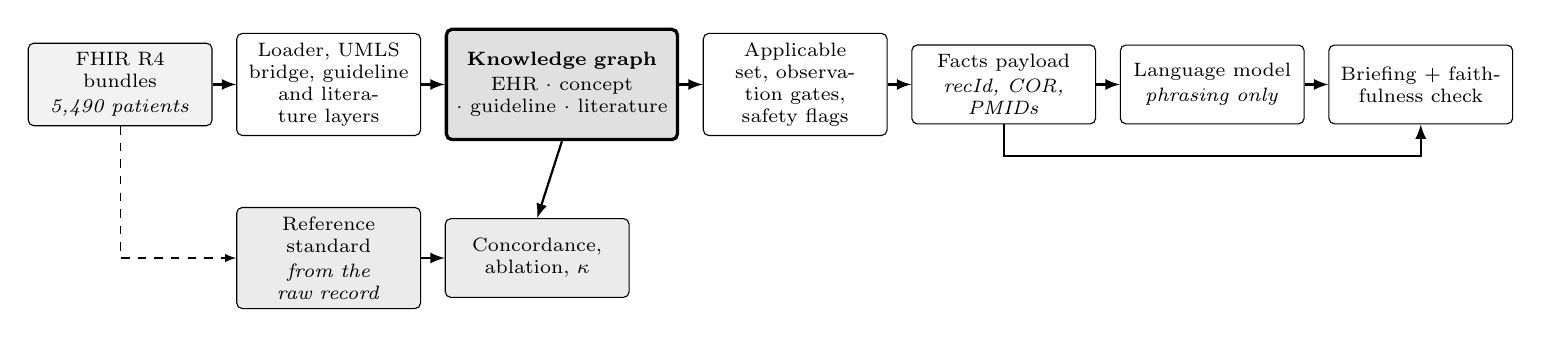
\begin{tikzpicture}[
    node distance = 7mm and 3mm,
    box/.style   = {rectangle, rounded corners=2pt, draw, text width=21mm,
                    align=center, minimum height=10mm, font=\scriptsize},
    src/.style   = {box, fill=black!5},
    ev/.style    = {box, fill=black!8},
    store/.style = {rectangle, rounded corners=2pt, draw, very thick, fill=black!12,
                    text width=27mm, align=center, minimum height=14mm, font=\scriptsize},
    ar/.style    = {-latex, thick},
    raw/.style   = {-latex, dashed},
    lbl/.style   = {font=\tiny, inner sep=1pt}
]
\node[src] (s) {FHIR R4 bundles\\[1pt]\emph{5{,}490 patients}};
\node[box, right=of s] (b) {Loader, UMLS bridge, guideline and literature layers};
\node[store, right=of b] (g) {\textbf{Knowledge graph}\\[1pt]EHR $\cdot$ concept\\
      $\cdot$ guideline $\cdot$ literature};
\node[box, right=of g] (q) {Applicable set, observation gates, safety flags};
\node[box, right=of q] (f) {Facts payload\\[1pt]\emph{recId, COR, PMIDs}};
\node[box, right=of f] (l) {Language model\\[1pt]\emph{phrasing only}};
\node[box, right=of l] (o) {Briefing + faithfulness check};

\node[ev, below=9mm of b] (ref) {Reference standard\\[1pt]\emph{from the raw record}};
\node[ev, right=of ref] (ev) {Concordance, ablation, $\kappa$};

\draw[ar] (s) -- (b);
\draw[ar] (b) -- (g);
\draw[ar] (g) -- (q);
\draw[ar] (q) -- (f);
\draw[ar] (f) -- (l);
\draw[ar] (l) -- (o);
\draw[ar] (f.south) -- ++(0,-4mm) -| (o.south);
\draw[raw] (s.south) |- (ref.west);
\draw[ar] (ref) -- (ev);
\draw[ar] (g.south) -- (ev.north);
\end{tikzpicture}}
\caption{System architecture. The build runs once and writes a single store; every
per-patient query reads that same store, and the language model receives only what
deterministic retrieval has already assembled. The dashed arrow is the separate data path:
the reference standard is computed from the raw record, never from the graph the system
under test queries.}
\label{fig:arch}
\end{figure*}

\subsection{Graph Construction}
Each FHIR resource becomes a node carrying both a structural \texttt{:Resource} label and
its resource-type label, each reference becomes a relationship typed after the element it
came from (\texttt{Observation.subject} yields a \texttt{SUBJECT} edge rather than a
generic one), and each terminology code becomes a shared \texttt{:Code} node keyed on
(system,~code). Every write is a \texttt{MERGE}, so reloading a bundle cannot duplicate a
node, a code or an edge. Patient records are synthetic, generated by Synthea
\cite{synthea,walonoski2017}, so the full record can be published alongside the code.

\subsection{Terminology Bridge}
The deduplicated code universe is exported from the graph and mapped to UMLS concept
unique identifiers by a three-pass linker built on scispaCy \cite{scispacy}. Because the
export is taken \emph{from the graph} rather than from the source files, the bridge links
exactly the codes the graph actually holds. A \texttt{:Concept} node then joins to
\texttt{:Code} by a \texttt{SAME\_CONCEPT} edge, and a patient is matched to a guideline
concept by the traversal \texttt{(p)<-[:SUBJECT]-(:Condition)-[:CODE]->(:Code)
<-[:SAME\_CONCEPT]-(:Concept)}.

\subsection{Guideline and Literature Layers}
Guideline recommendations are loaded as \texttt{:Recommendation} nodes carrying a class of
recommendation, with \texttt{TARGETS}, \texttt{RECOMMENDS} and \texttt{CONTRAINDICATES}
edges into the concept space. The literature layer holds 4,801 PubMed abstracts seeded from
the guideline's own reference list, with entity mentions linked to concepts and
co-occurrence edges weighted by pointwise mutual information \cite{pmi}.

\subsection{Observation Gates}
Several recommendations are conditioned not on the presence of a condition but on a
measured value---a beta-blocker recommendation on left-ventricular ejection fraction, a
weight-management recommendation on body-mass index. A condition-only pipeline cannot
express these and must fire them for every cohort member. Because numeric observations are
loaded into the graph, each such recommendation is instead paired with a predicate over
graph-derived features. The predicate \emph{overrides} the graph's gate-and-\texttt{AND}
decision rather than intersecting with it, so a disjunctive precondition adds patients
rather than being filtered out by a blanket conjunction. The thresholds and aggregation
rules are the reference standard's own, which bears on how the ablation can be read
(Section~\ref{sec:eval}).

\subsection{Grounded Briefing}
The briefing is produced in four stages: deterministic Cypher retrieval of the patient
snapshot, applicable recommendations, safety flags and literature support; assembly into a
structured facts payload in which every item carries its provenance; a single
language-model call constrained to phrase those facts; and emission of the facts and the
text as separate artifacts so that faithfulness can be checked mechanically. The model has
no path back to the graph, so any recommendation it names beyond what retrieval supplied is
necessarily fabricated, and the check detects it.

\section{Evaluation Design}
\label{sec:eval}

Evaluation covers 876 CCD patients. Labels are produced by a separate module that reads the
\emph{raw FHIR bundles}---never Neo4j and never the system's output---and applies the
guideline logic directly. That separation holds for the data path of every recommendation,
but how independent the reference is differs by tier. For 53 of the 68 scored
recommendations the two sides also differ in logic: the system decides by graph traversal
over UMLS-bridged codes, the reference by string matching over the condition names in the
bundle. For the 15 observation-gated recommendations the gate reuses the reference
standard's thresholds and aggregations, so the two predicates are the same function. This
was checked rather than assumed: over the 876 real feature vectors and 200,000 synthetic ones
aimed at every threshold, missing values included, the two never disagree. For those 15,
agreement shows that the loader carries patient values unchanged, not that the thresholds
are clinically right.

This automatically generated \emph{silver} standard is itself validated against a
\emph{gold} standard of 30 patients labelled manually by the author from the full record,
the standard justification for substituting generated labels for manual annotation at
scale \cite{rebholz2011,nogues2022}. Agreement is reported as Cohen's $\kappa$
\cite{cohen1960}, with a 95\% confidence interval from a 10,000-replicate bootstrap
\cite{efron1994} that resamples patients rather than cells, since one record determines
all of a patient's labels \cite{field2007}; prevalence and bias indices and PABAK are
reported alongside \cite{byrt1993}.

The observation-gate ablation compares two arms that share the same baseline and differ
only in whether the observation predicates are applied, so the difference isolates the
contribution of the gate itself, not of the data container. A third arm tests the
container: the same gate is rebuilt from Synthea's CSV export alone, with its logic copied
verbatim from the reference module, and its decisions are compared with the bundle path.

Briefings for the 30 gold-standard patients are checked automatically for four things:
every cited recommendation identifier and every cited PMID must be in the facts, every
applicable recommendation and safety flag must be mentioned, and the text must not claim
that the patient requires oral anticoagulation when none is on the medication list.

The tiers so far test the system against rules derived from the guideline. A clinician
review tests whether its recommendations suit the patient. Twenty of the 30 sample patients
were presented one per page, with the briefing's conclusion (in an Indonesian translation
lightly edited by the author) and a table of 327 recommendations: every safety flag and
every applicable recommendation triggered by the patient's own conditions. Each row was
rated \emph{appropriate}, \emph{not yet appropriate} or \emph{cannot be judged}, with a
comment for the last two. Three clinicians rated independently but only in part: a
cardiologist (rater~A) rated patients 1--15, a general practitioner (rater~B) patients
1--10, and a senior cardiologist (rater~C) patient~1. Proportions carry per-patient
bootstrap intervals, and agreement between raters~A and~B on their shared rows is reported
as three-category $\kappa$ and PABAK.

Graph quality is reported along the
structural dimensions of ontology evaluation \cite{gangemi2006}, with richness after OntoQA
\cite{tartir2005} and width corresponding to the completeness dimension of knowledge-graph
quality \cite{issa2021}; because a property graph has no subsumption hierarchy, richness is
reported as counts rather than as OntoQA's ratios.

\section{Results}

\subsection{Graph Scale and Structure}
The constructed graph contains 1,804,379 nodes and 8,796,425 relationships over 25 node
labels, 51 relationship types and 26 code systems. The \texttt{:Patient} count equals the
number of patients Synthea reported generating, confirming that the idempotent load neither
dropped nor duplicated a record.

\subsection{Observation-Gate Ablation}
Gating raises guideline concordance $F_1$ from 0.743 to 0.810, a gain of $+0.067$ obtained
through precision (0.612 to 0.684) with recall essentially unchanged (0.948 to 0.994).
Table~\ref{tab:ablation} decomposes this by how a recommendation discriminates: whether it
requires a further condition target, a numeric predicate, both, or neither.

\begin{table}[htbp]
\caption{Concordance by discrimination class in both ablation arms, micro-averaged over
876 patients}
\label{tab:ablation}
\begin{center}
\setlength{\tabcolsep}{3.5pt}
\begin{tabular}{|l|c|c c c|c c c|}
\hline
\textbf{Class} & \textbf{recs} & \multicolumn{3}{c|}{\textbf{Baseline}}
                               & \multicolumn{3}{c|}{\textbf{With gates}} \\
\cline{3-8}
 & & \textbf{P} & \textbf{R} & \textbf{$F_1$}
   & \textbf{P} & \textbf{R} & \textbf{$F_1$} \\
\hline
Universal        & 38 & 0.666 & 1.000 & 0.799 & 0.666 & 1.000 & 0.799 \\
Concept-matched  & 15 & 0.676 & 0.915 & 0.777 & 0.676 & 0.915 & 0.777 \\
Value-gated      & 5  & 0.194 & 1.000 & 0.325 & \textbf{1.000} & \textbf{1.000} & \textbf{1.000} \\
Both             & 10 & 0.038 & 0.006 & 0.011 & \textbf{1.000} & \textbf{1.000} & \textbf{1.000} \\
\hline
\textbf{All}     & 68 & 0.613 & 0.945 & 0.743 & 0.685 & 0.993 & 0.811 \\
\hline
\end{tabular}
\end{center}
\end{table}

Two results follow, neither visible in the aggregate. First, the two ungated classes are
\emph{identical} across the arms---not merely close, but equal to the individual
true-positive, false-positive and false-negative counts. Fifty-three of the 68
recommendations are therefore untouched, and the whole of the reported difference
originates in the remaining 15. This is a falsifiable prediction of the classification, and
it holds exactly.

Second, the two gated classes benefit in \emph{opposite} ways. For the five
\emph{value-gated} recommendations, gating is a precision mechanism: without it they fire
for every cohort member ($P = 0.194$), and with it only where the measured value satisfies
the predicate, while recall was already perfect. For the ten in the \emph{both} class,
gating is overwhelmingly a \emph{recall} mechanism: in the baseline arm they almost never
fire at all ($R = 0.006$), because their encoded condition targets alone rarely match and
the numeric predicate is what identifies the patients they apply to. Describing the
ablation solely as a precision improvement, as the aggregate invites, is therefore
incorrect for two thirds of the affected recommendations.

Both gated classes reach $P = R = 1.000$ once gating is enabled. They are exactly the 15
recommendations whose predicate the gate shares with the reference standard, so this
establishes that the loader preserved the observation values, not that the thresholds are
clinically right: the ablation gain measures implementation fidelity rather than clinical
validity. The part scored by a genuinely independent judge, the other 53 recommendations,
reaches $P = 0.666$ and $F_1 = 0.797$ against 0.685 and 0.811 for all 68. The headline
figure is therefore not propped up by the shared part.

The table is micro-averaged, and the choice matters. Macro-averaging over patients scores a
patient a class never touches as a complete failure, because with no reference label and no
system output precision, recall and $F_1$ are defined as zero rather than left undefined.
The value-gated class shows the distortion at full size: macro $F_1 = 0.600$ against a micro
value of 1.000, the macro figure being nothing but the share of the cohort---526 of the
876---that carries a value-gated recommendation at all.

\subsection{Does the Gain Require FHIR?}
Rebuilt from the CSV export, the gate reproduces all 2,120 true positives with no false
positive or negative: not one of 13,140 decisions (876 patients times 15 recommendations)
differs from the bundle path, and SNOMED~CT code \texttt{414545008} in
\texttt{conditions.csv} selects the same 876 patients. Two losses are measurable, and
neither changes a decision. The export rounds values to one decimal place, moving 1,990
values by at most 0.05. Three cross a threshold: an ejection fraction of 39.999 that becomes
40.0, which the predicates ``$\le 40$'' and ``$> 40$'' answer identically either way, and
two triglyceride values whose recommendation also requires an LDL the patients do not meet. The blood-pressure panel is split into separate rows, but the
\texttt{ENCOUNTER} key reassembles all 17,177 systolic--diastolic pairs. The gain therefore
comes from loading numeric observations as first-class data; FHIR is the most direct route
to them, not the only one. The result holds for an export that carries such a key and does
not make tabular exports and FHIR equivalent in general.

\subsection{Silver--Gold Agreement}
On the 30 manually labelled patients, the silver standard agrees on 99.5\% of cells (2,150
of 2,160) with Cohen's $\kappa = 0.991$. Resampling patients and resampling cells give the
same 95\% interval, 0.984--0.996: the ten disagreements fall on 8 patients, none
contributing more than two, and the design effect is 1.04. Positive labels cover 50.2\% of
cells and the disagreements split five and five, so $\kappa$ is not inflated by prevalence
and equals PABAK. The lower bound sits well above the 0.80 threshold for near-perfect
agreement \cite{landis1977}, which 30 patients suffice to support; they would not support a
finer claim. Because the generated standard reproduces human judgement almost exactly where
both exist, the concordance figures computed over the full cohort rest on a validated
reference rather than an assumed one. The gold standard has a single annotator, a limitation
that resampling cannot address.

\subsection{Contraindication Safety}
Table~\ref{tab:safety} reports safety detection over 151 manually labelled flags. The
result is a genuine trade-off rather than a tunable failure: unary matching never misses a
reachable contraindication but over-flags heavily, whereas population gating is perfectly
precise but recovers only those contraindications whose population condition is
structurally gateable. The misses are the negation-defined and conjunctive
contraindications that a flat schema cannot express.

\begin{table}[htbp]
\caption{Contraindication-safety detection}
\label{tab:safety}
\begin{center}
\begin{tabular}{|l|c|c|c|}
\hline
\textbf{Variant} & \textbf{P} & \textbf{R} & \textbf{$F_1$} \\
\hline
Unary (contraindicated drug alone) & 0.139 & $\approx$1.000 & --- \\
Population-gated (drug \emph{and} condition) & 1.000 & 0.095 & 0.174 \\
Chronicity-gated (\texttt{APT:10} only) & 0.909 & 0.526 & 0.667 \\
\hline
\end{tabular}
\end{center}
\end{table}

\subsection{Briefing Faithfulness}
All 30 briefings pass all four checks: zero fabricated recommendations, zero fabricated
PMIDs, zero omitted recommendations and zero anticoagulation over-claims. The fourth check
needs its history. Its first run flagged 10 lines in 4 briefings, all false positives of one
shape: the provenance trace wrote ``conditional on oral anticoagulation need'', and the
pattern matched \emph{on}. The check was then restricted to the parts of the briefing a
reader acts on, a correction made after the output was seen. These checks are not semantic
faithfulness. Deterministic retrieval makes the facts exact and the citable items checkable
against a closed set, but the model can still attach a condition that is not in the facts,
misstate why a recommendation applies, or present a weak recommendation as mandatory, and
apart from the anticoagulation pattern none of this is caught. What is established is
citation-level and completeness faithfulness.

\subsection{Clinician Review}
Table~\ref{tab:clinician} summarises the ratings. Rater~A judged 77.7\% of recommendations
appropriate (95\% per-patient CI 74.4--81.1\%), rater~B 60.6\% (56.1--67.3\%); excluding
\emph{cannot be judged}, the two are close, at 78.7\% and 74.6\%.

\begin{table}[htbp]
\caption{Clinician ratings of the system's recommendations}
\label{tab:clinician}
\begin{center}
\setlength{\tabcolsep}{3pt}
\begin{tabular}{|l|c|c|c|c|c|}
\hline
\textbf{Rater} & \textbf{Patients} & \textbf{Rows} & \textbf{Approp.} & \textbf{Not yet}
               & \textbf{Cannot} \\
\hline
A (cardiologist)        & 1--15 & 247 & 77.7\% & 21.1\% & 1.2\%  \\
B (general practitioner) & 1--10 & 160 & 60.6\% & 20.6\% & 18.8\% \\
C (senior cardiologist) & 1     & 16  & 6      & 5      & 5      \\
\hline
\end{tabular}
\end{center}
\end{table}

Appropriateness is uneven. Outside the antithrombotic and beta-blocker recommendations,
rater~A judged 105 of 106 rows appropriate and rater~B all 69, including the three
shared-predicate recommendations on the sheet, whose 50 ratings are all appropriate---a
small independent test of rules the reference standard shares. Most \emph{not yet
appropriate} ratings fall on antithrombotic recommendations: 46 of rater~A's 52 and 32 of
rater~B's 33. Raters~A and~B agree on 65.4\% of their 159 shared rows ($\kappa = 0.29$,
95\% CI 0.18--0.41; PABAK 0.48), fair agreement \cite{landis1977}, but 98.6\% outside the
antithrombotic and beta-blocker rows and 40.0\% inside them. On beta-blocker rows almost all
the disagreement is rater~B's \emph{cannot be judged}, asking for ejection fraction and
heart-failure status. On antithrombotic rows rater~B proposed a different anticoagulant
sequence, and rater~A rejected 13 of 15 flags to stop clopidogrel. The two groups share a
dependence on information the conclusion did not present: time since an acute coronary
syndrome, bleeding risk, the indication for anticoagulation, ejection fraction and
heart-failure status. Rater~C's comments expose the same limit: two flagged drugs were
judged unassessable because the conclusion did not name them, although both are in the
record.

\section{Discussion}

The central claim of this work is supported, in a narrower form than first stated. Loading
numeric observations as first-class data makes a measurable contribution to the precision of
guideline concordance; the ablation localises that contribution exactly and shows it to be
two mechanisms rather than one. FHIR supplies those observations most directly, but the
tabular export reproduces the same gate, so the claim is that numeric observations are
necessary, not that FHIR is.

A second finding was not anticipated and bears on any FHIR-based deployment. The two
projections of the same synthetic record are not comparable in richness: the FHIR export
retains a categorical medication status but omits stop dates, while the paired CSV export
retains stop dates but carries no status, so neither is a superset of the other. The
chronic-NSAID rule depends on how long a drug was taken, and consequently only two of its
four arms can be computed from the graph. The cost is measured rather than hypothetical, as
the chronicity-gated row of Table~\ref{tab:safety} shows: precision 0.909 at recall 0.526,
missing exactly those patients whose use is chronic only through a single long course. A
system consuming FHIR alone must anticipate this class of information loss wherever a
guideline depends on exposure duration.

The clinician review points to the same place as the residual false positives:
recommendations whose preconditions structured data cannot confirm. It also shows what the
briefing should state---the flagged drugs and the values a recommendation rests on, or
that they are unknown---since their absence is what most often prevented a judgement.

Several limitations bound the results. The records are synthetic, so the figures establish
that the pipeline is internally correct rather than that it would perform equally on real
records, which are noisier and sparser; they also carry no cardiac symptoms, so six
angina-dependent recommendations were never exercised. The cohort gate accepts a single
UMLS concept whereas the guideline defines CCD disjunctively, so 7.1\% of the clinically
defined cohort, whose only evidence is a prior-infarction or prior-revascularization
\emph{situation} code, is never matched against any recommendation; widening the gate is a
small query change and the first item of future work. The gold standard has one annotator,
who also encoded the reference rules. For the 15 shared-predicate recommendations the
ablation measures implementation fidelity, not clinical validity. The clinician review is
partial---one cardiologist across 15 patients, fair agreement between raters, and raters
who read only the conclusion---so it locates weak points rather than estimating clinical
appropriateness in general. And semantic faithfulness remains unchecked: a reader study on
the model of Van~Veen \textit{et al.}~\cite{vanveen2023}, scoring completeness, correctness
and conciseness with inter-rater agreement, is still the natural next step.

\section{Conclusion}

This paper presented a FHIR-native, knowledge-graph-based clinical recommendation system for
chronic coronary disease that fuses the patient record, a clinical guideline and a
literature corpus through a UMLS concept bridge. Observation gating, made possible by
loading numeric observations as graph data, raises guideline concordance $F_1$ from 0.743
to 0.810, with the entire gain confined to the 15 of 68 recommendations that are gated and
acting through precision for one gated class and recall for the other; a tabular export
reproduces the same gate, so the gain belongs to the numeric observations rather than to
FHIR itself. The reference standard is computed from the raw record and validated at
$\kappa = 0.991$ (95\% CI 0.984--0.996). Deterministic retrieval makes the citation-level
faithfulness of the briefing decidable, though not the meaning of every sentence. A
clinician review judged most recommendations appropriate and located the weak point in
antithrombotic therapy, where the guideline depends on information the briefing does not
yet present. The design thus offers guideline-concordant support whose claims can be
checked rather than trusted, within limits that are themselves measured.

\section*{Acknowledgment}

<<Acknowledgment.>>

\bibliographystyle{IEEEtran}
\bibliography{references}

\end{document}
